\documentclass{beamer}

% Theme selection - auto-detect UASLP1 or fallback to Madrid
\IfFileExists{beamerthemeUASLP1.sty}{
    \usetheme{UASLP1}
}{
    \usetheme{Madrid}
    \usecolortheme{seahorse}
}

% Packages
\usepackage[utf8]{inputenc}
\usepackage[T1]{fontenc}
\usepackage{lmodern}
\usepackage{tikz}
\usepackage{listings}
\usepackage{xcolor}
\usepackage{amsmath}
\usepackage{hyperref}

% TikZ libraries
\usetikzlibrary{shapes.geometric, arrows.meta, positioning, fit, backgrounds}

% Code listing style
\lstset{
    language=C,
    basicstyle=\ttfamily\small,
    keywordstyle=\color{blue}\bfseries,
    commentstyle=\color{green!60!black}\itshape,
    stringstyle=\color{red},
    showstringspaces=false,
    breaklines=true,
    frame=single,
    numbers=left,
    numberstyle=\tiny\color{gray},
    tabsize=2,
    captionpos=b
}

% Title information
\title[USP Course 5: Hardware Integration]{Course 5: Hardware Integration}
\subtitle{USP Training Series}
\author{USP Development Team}
\institute{Universal Software Platform}
\date{\today}

\begin{document}

% Title slide
\begin{frame}
\titlepage
\end{frame}

% Table of contents
\begin{frame}{Course Overview}
\tableofcontents
\end{frame}

% ============================================================================
\section{Introduction}
% ============================================================================

\begin{frame}{Course 5: Hardware Integration}
\begin{block}{Learning Objectives}
\begin{itemize}
    \item Configure device tree for custom hardware
    \item Calibrate TX power for regulatory compliance
    \item Port HAL to new MCU platforms
    \item Adapt USP to custom board designs
    \item Integrate custom sensors and peripherals
\end{itemize}
\end{block}

\vspace{0.5cm}

\begin{block}{Hands-On Labs}
\begin{itemize}
    \item Lab 5.1: Device Tree Configuration
    \item Lab 5.2: TX Power Calibration
    \item Lab 5.3: Custom Board HAL Port
\end{itemize}
\end{block}
\end{frame}

\begin{frame}{Prerequisites}
\begin{itemize}
    \item Completion of Courses 1-4
    \item Understanding of Zephyr RTOS device tree
    \item Familiarity with GPIO, SPI, I2C protocols
    \item Knowledge of LR1120/LR1121 radio configuration
    \item Access to test equipment (spectrum analyzer, power meter)
\end{itemize}

\vspace{0.5cm}

\begin{alertblock}{Hardware Required}
Custom board or development kit different from Xiao nRF54L15
\end{alertblock}
\end{frame}

\begin{frame}{Why Hardware Integration Matters}
\begin{columns}
\column{0.5\textwidth}
\textbf{Production Deployment:}
\begin{itemize}
    \item Custom PCB designs
    \item Different MCU/radio combinations
    \item Cost optimization
    \item Form factor requirements
    \item Specific peripheral needs
\end{itemize}

\vspace{0.3cm}

\textbf{Regulatory Compliance:}
\begin{itemize}
    \item TX power accuracy
    \item Frequency accuracy
    \item Spurious emissions
    \item Certification testing
\end{itemize}

\column{0.5\textwidth}
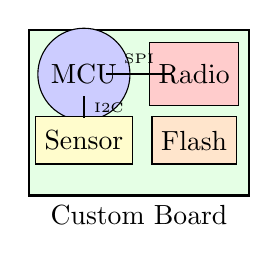
\begin{tikzpicture}[scale=0.7]
    % Custom board representation
    \draw[thick, fill=green!10] (0,0) rectangle (4,3);

    % Components
    \node[draw, circle, fill=blue!20, minimum size=0.8cm] at (1,2.2) {MCU};
    \node[draw, rectangle, fill=red!20, minimum size=0.8cm] at (3,2.2) {Radio};
    \node[draw, rectangle, fill=yellow!20, minimum size=0.6cm] at (1,1) {Sensor};
    \node[draw, rectangle, fill=orange!20, minimum size=0.6cm] at (3,1) {Flash};

    % Labels
    \node[below] at (2,0) {Custom Board};

    % Connections
    \draw[thick] (1.4,2.2) -- (2.6,2.2) node[midway, above] {\tiny SPI};
    \draw[thick] (1,1.8) -- (1,1.4) node[midway, right] {\tiny I2C};
\end{tikzpicture}
\end{columns}
\end{frame}

% ============================================================================
\section{Device Tree Configuration}
% ============================================================================

\begin{frame}{Zephyr Device Tree Overview}
\begin{block}{What is Device Tree?}
Device Tree (DT) is a hardware description format used by Zephyr to configure:
\begin{itemize}
    \item GPIO pin assignments
    \item SPI/I2C bus configuration
    \item Peripheral properties
    \item Board-specific settings
\end{itemize}
\end{block}

\vspace{0.3cm}

\textbf{Key Files:}
\begin{itemize}
    \item \texttt{boards/arm/myboard/myboard.dts} -- Main board definition
    \item \texttt{boards/arm/myboard/myboard.overlay} -- Application overlay
    \item \texttt{dts/bindings/} -- Device bindings (schema)
\end{itemize}

\vspace{0.3cm}

\textbf{Syntax:}
\begin{itemize}
    \item Hierarchical node structure
    \item Properties: \texttt{property = <value>;}
    \item References: \texttt{\&label}
\end{itemize}
\end{frame}

\begin{frame}[fragile]{Device Tree Structure}
\begin{lstlisting}[language=bash, caption={Example Device Tree}]
/ {
    model = "My Custom Board";
    compatible = "vendor,myboard";

    chosen {
        zephyr,console = &uart0;
        zephyr,shell-uart = &uart0;
    };

    leds {
        compatible = "gpio-leds";
        led0: led_0 {
            gpios = <&gpio0 13 GPIO_ACTIVE_LOW>;
            label = "Status LED";
        };
    };

    buttons {
        compatible = "gpio-keys";
        button0: button_0 {
            gpios = <&gpio0 11 GPIO_ACTIVE_LOW>;
            label = "User Button";
        };
    };
};
\end{lstlisting}
\end{frame}

\begin{frame}[fragile]{Configure SPI Bus for LR1120}
\begin{lstlisting}[language=bash, caption={SPI and GPIO Configuration}]
&spi2 {
    compatible = "nordic,nrf-spim";
    status = "okay";
    cs-gpios = <&gpio0 8 GPIO_ACTIVE_LOW>;

    lr1120: lr1120@0 {
        compatible = "semtech,lr1120";
        reg = <0>;
        spi-max-frequency = <16000000>;

        reset-gpios = <&gpio0 14 GPIO_ACTIVE_LOW>;
        busy-gpios = <&gpio0 15 GPIO_ACTIVE_HIGH>;
        dio1-gpios = <&gpio0 28 GPIO_ACTIVE_HIGH>;

        // TX power configuration
        tx-power-offset = <2>;  // dB
        antenna-gain = <0>;     // dBi

        // Frequency calibration
        freq-error-hz = <0>;
    };
};
\end{lstlisting}
\end{frame}

\begin{frame}[fragile]{Device Tree Overlays}
\begin{block}{What are Overlays?}
Overlays allow application-specific modifications without changing base board definition.
\end{block}

\vspace{0.3cm}

\begin{lstlisting}[language=bash, caption={myapp.overlay}]
// Add sensor on I2C bus
&i2c0 {
    bme680: bme680@76 {
        compatible = "bosch,bme680";
        reg = <0x76>;
        label = "BME680";
    };
};

// Disable unused peripherals to save power
&uart1 {
    status = "disabled";
};

&pwm0 {
    status = "disabled";
};
\end{lstlisting}
\end{frame}

\begin{frame}{Device Tree Pin Assignment}
\begin{center}
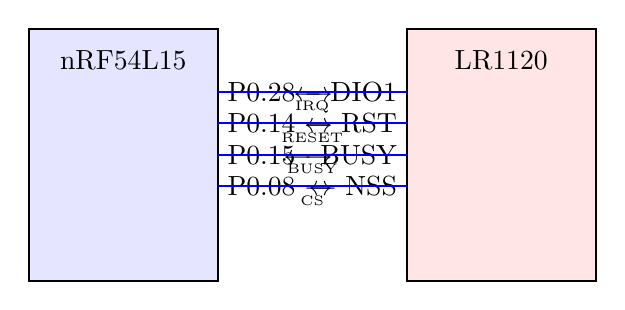
\begin{tikzpicture}[scale=0.8]
    % MCU
    \draw[thick, fill=blue!10] (0,0) rectangle (3,4);
    \node at (1.5,3.5) {nRF54L15};

    % Pins on MCU
    \node[right] at (3,3) {P0.28 $\rightarrow$};
    \node[right] at (3,2.5) {P0.14 $\rightarrow$};
    \node[right] at (3,2) {P0.15 $\rightarrow$};
    \node[right] at (3,1.5) {P0.08 $\rightarrow$};

    % LR1120
    \draw[thick, fill=red!10] (6,0) rectangle (9,4);
    \node at (7.5,3.5) {LR1120};

    % Pins on LR1120
    \node[left] at (6,3) {$\leftarrow$ DIO1};
    \node[left] at (6,2.5) {$\leftarrow$ RST};
    \node[left] at (6,2) {$\leftarrow$ BUSY};
    \node[left] at (6,1.5) {$\leftarrow$ NSS};

    % Connections
    \draw[thick, blue] (3,3) -- (6,3);
    \draw[thick, blue] (3,2.5) -- (6,2.5);
    \draw[thick, blue] (3,2) -- (6,2);
    \draw[thick, blue] (3,1.5) -- (6,1.5);

    % Labels
    \node[below] at (4.5,3) {\tiny IRQ};
    \node[below] at (4.5,2.5) {\tiny RESET};
    \node[below] at (4.5,2) {\tiny BUSY};
    \node[below] at (4.5,1.5) {\tiny CS};
\end{tikzpicture}
\end{center}

\vspace{0.3cm}

\textbf{Pin Assignment Considerations:}
\begin{itemize}
    \item Use GPIO pins that support required functions
    \item Avoid conflicts with other peripherals
    \item Consider power domain and voltage levels
    \item Check MCU datasheet for restrictions
\end{itemize}
\end{frame}

% ============================================================================
\section{TX Power Calibration}
% ============================================================================

\begin{frame}{Why TX Power Calibration?}
\begin{block}{Regulatory Requirements}
\begin{itemize}
    \item EU868: Maximum +14 dBm EIRP (typical)
    \item US915: Maximum +30 dBm EIRP
    \item AS923: Maximum +16 dBm EIRP
    \item Varies by frequency sub-band
\end{itemize}
\end{block}

\vspace{0.3cm}

\textbf{System Factors Affecting TX Power:}
\begin{enumerate}
    \item Radio output power (LR1120: -17 to +22 dBm)
    \item PCB trace losses (typically 0.5-1 dB)
    \item Antenna matching network losses (0.5-2 dB)
    \item Antenna gain (0 to +3 dBi typical)
\end{enumerate}

\vspace{0.3cm}

\[
\text{EIRP} = P_{radio} - L_{traces} - L_{matching} + G_{antenna}
\]
\end{frame}

\begin{frame}{TX Power Calibration Setup}
\begin{columns}
\column{0.5\textwidth}
\textbf{Required Equipment:}
\begin{itemize}
    \item Spectrum analyzer
    \item RF power meter
    \item 50$\Omega$ dummy load
    \item SMA cables
    \item RF attenuators (20-30 dB)
\end{itemize}

\vspace{0.3cm}

\textbf{Procedure:}
\begin{enumerate}
    \item Set radio to CW mode
    \item Measure output power
    \item Calculate offset
    \item Update device tree
    \item Verify compliance
\end{enumerate}

\column{0.5\textwidth}
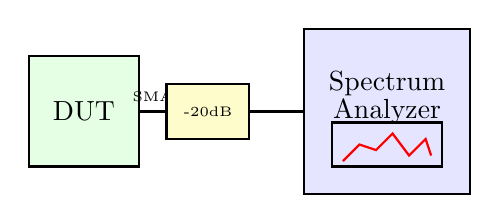
\begin{tikzpicture}[scale=0.7]
    % DUT (Device Under Test)
    \draw[thick, fill=green!10] (0,2) rectangle (2,4);
    \node at (1,3) {DUT};

    % Antenna connector
    \draw[thick] (2,3) -- (2.5,3);
    \node[above] at (2.25,3) {\tiny SMA};

    % Attenuator
    \draw[thick, fill=yellow!20] (2.5,2.5) rectangle (4,3.5);
    \node at (3.25,3) {\tiny -20dB};

    % Cable
    \draw[thick] (4,3) -- (5,3);

    % Spectrum analyzer
    \draw[thick, fill=blue!10] (5,1.5) rectangle (8,4.5);
    \node at (6.5,3.5) {Spectrum};
    \node at (6.5,3) {Analyzer};

    % Screen representation
    \draw[thick] (5.5,2) rectangle (7.5,2.8);
    \draw[thick, red] (5.7,2.1) -- (6,2.4) -- (6.3,2.3) -- (6.6,2.6) -- (6.9,2.2) -- (7.2,2.5) -- (7.3,2.2);
\end{tikzpicture}
\end{columns}
\end{frame}

\begin{frame}[fragile]{Measure TX Power}
\begin{lstlisting}[caption={Test Firmware for Calibration}]
#include <lr11xx_radio.h>
#include <lr11xx_system.h>

void tx_power_calibration_mode(void) {
    // Set to CW (Continuous Wave) mode
    lr11xx_radio_set_rf_freq(868100000);  // 868.1 MHz

    // Set PA config
    lr11xx_radio_pa_cfg_t pa_cfg = {
        .pa_sel = LR11XX_RADIO_PA_SEL_HP,
        .pa_reg_supply =
            LR11XX_RADIO_PA_REG_SUPPLY_VBAT,
        .pa_duty_cycle = 0x04,
        .pa_hp_sel = 0x07,
    };
    lr11xx_radio_set_pa_cfg(&pa_cfg);

    // Set output power (register value)
    lr11xx_radio_set_tx_params(14,
        LR11XX_RADIO_RAMP_48_US);  // +14 dBm

    // Enable CW transmission
    lr11xx_radio_set_tx_cw();

    // Measure output power on spectrum analyzer
    // Note actual power, calculate offset
}
\end{lstlisting}
\end{frame}

\begin{frame}{TX Power Offset Calculation}
\begin{block}{Example Measurement}
\begin{itemize}
    \item Radio configured for: +14 dBm
    \item Measured output (with 20 dB attenuator): -7.5 dBm
    \item Actual output: -7.5 + 20 = +12.5 dBm
    \item Offset: 12.5 - 14 = -1.5 dB
\end{itemize}
\end{block}

\vspace{0.3cm}

\textbf{Typical Offset Sources:}
\begin{itemize}
    \item PCB losses: -0.5 dB
    \item Matching network: -0.8 dB
    \item Connector: -0.2 dB
    \item \textbf{Total: -1.5 dB} $\checkmark$
\end{itemize}

\vspace{0.3cm}

\begin{alertblock}{Apply Offset in Device Tree}
Add \texttt{tx-power-offset = <-2>;} to compensate\\
(rounded to nearest integer)
\end{alertblock}
\end{frame}

\begin{frame}[fragile]{Configure TX Power Offset}
\begin{lstlisting}[language=bash, caption={Device Tree TX Power Configuration}]
&spi2 {
    lr1120: lr1120@0 {
        compatible = "semtech,lr1120";
        reg = <0>;

        // Calibration results
        tx-power-offset = <-2>;  // dB compensation

        // Antenna characteristics
        antenna-gain = <2>;  // 2 dBi antenna

        // Regulatory limit (EU868)
        tx-power-max = <14>;  // EIRP limit

        // Per-band calibration (optional)
        tx-power-offset-868 = <-2>;
        tx-power-offset-915 = <-1>;
    };
};
\end{lstlisting}

\vspace{0.3cm}

Now when application requests +14 dBm, radio will be set to +16 dBm to compensate for -2 dB losses.
\end{frame}

\begin{frame}[fragile]{Frequency Accuracy Calibration}
\begin{columns}
\column{0.5\textwidth}
\textbf{Why Frequency Matters:}
\begin{itemize}
    \item LoRaWAN requires ±20 ppm
    \item Crystal tolerance varies
    \item Temperature affects frequency
    \item Regulatory compliance
\end{itemize}

\vspace{0.3cm}

\textbf{Measurement:}
\begin{enumerate}
    \item Transmit CW at 868 MHz
    \item Measure on spectrum analyzer
    \item Calculate error in Hz
    \item Apply correction
\end{enumerate}

\column{0.5\textwidth}
\textbf{Example:}
\begin{itemize}
    \item Target: 868.100 MHz
    \item Measured: 868.095 MHz
    \item Error: -5 kHz
    \item PPM: -5000/868100000 = -5.8 ppm
\end{itemize}

\vspace{0.3cm}

\begin{lstlisting}[language=bash]
&lr1120 {
    freq-error-hz = <-5000>;
};
\end{lstlisting}

\vspace{0.3cm}

Radio driver will compensate by adding 5 kHz to all frequencies.
\end{columns}
\end{frame}

% ============================================================================
\section{HAL Porting}
% ============================================================================

\begin{frame}{Hardware Abstraction Layer (HAL)}
\begin{block}{What is HAL?}
HAL provides a standard interface between radio driver and hardware-specific operations:
\begin{itemize}
    \item SPI communication
    \item GPIO control (reset, busy, IRQ)
    \item Timing functions (delays, timestamps)
    \item Power management
\end{itemize}
\end{block}

\vspace{0.3cm}

\begin{center}
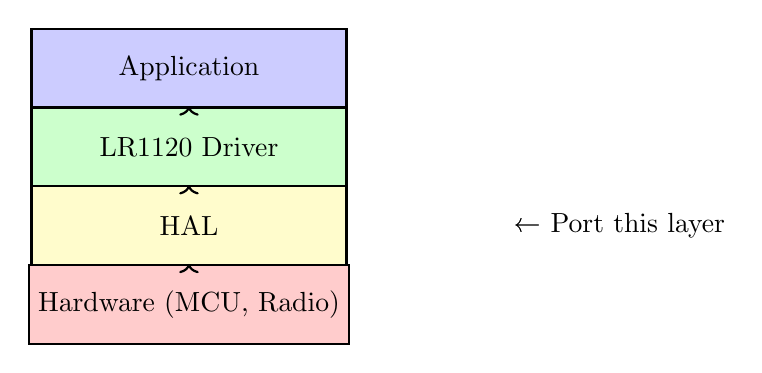
\begin{tikzpicture}[
    box/.style={rectangle, draw=black, thick, minimum height=1cm, minimum width=4cm, align=center}
]
    \node[box, fill=blue!20] (app) at (0,3) {Application};
    \node[box, fill=green!20] (driver) at (0,2) {LR1120 Driver};
    \node[box, fill=yellow!20] (hal) at (0,1) {HAL};
    \node[box, fill=red!20] (hw) at (0,0) {Hardware (MCU, Radio)};

    \draw[->, thick] (app) -- (driver);
    \draw[->, thick] (driver) -- (hal);
    \draw[->, thick] (hal) -- (hw);

    \node[right] at (4,1) {← Port this layer};
\end{tikzpicture}
\end{center}
\end{frame}

\begin{frame}[fragile]{HAL SPI Interface}
\begin{lstlisting}[caption={SPI HAL Functions}]
// Initialize SPI bus
int hal_spi_init(const struct device *spi_dev);

// SPI write transaction
int hal_spi_write(const struct device *spi_dev,
                  const uint8_t *data,
                  size_t len);

// SPI read transaction
int hal_spi_read(const struct device *spi_dev,
                 uint8_t *data,
                 size_t len);

// SPI write-then-read (typical for radio)
int hal_spi_write_read(const struct device *spi_dev,
                       const uint8_t *tx_data,
                       uint8_t *rx_data,
                       size_t len);
\end{lstlisting}
\end{frame}

\begin{frame}[fragile]{HAL GPIO Interface}
\begin{lstlisting}[caption={GPIO HAL Functions}]
// Configure GPIO pin
int hal_gpio_init(const struct gpio_dt_spec *gpio,
                  gpio_flags_t flags);

// Set GPIO output level
int hal_gpio_set(const struct gpio_dt_spec *gpio,
                 int value);

// Read GPIO input level
int hal_gpio_get(const struct gpio_dt_spec *gpio);

// Configure GPIO interrupt
int hal_gpio_interrupt_configure(
    const struct gpio_dt_spec *gpio,
    gpio_flags_t flags,
    gpio_callback_handler_t handler);

// Enable/disable GPIO interrupt
int hal_gpio_interrupt_enable(
    const struct gpio_dt_spec *gpio,
    bool enable);
\end{lstlisting}
\end{frame}

\begin{frame}[fragile]{HAL Timing Interface}
\begin{lstlisting}[caption={Timing HAL Functions}]
// Delay functions
void hal_delay_us(uint32_t microseconds);
void hal_delay_ms(uint32_t milliseconds);

// Timestamp functions (for ranging, etc.)
uint32_t hal_get_timestamp_us(void);
uint64_t hal_get_timestamp_ms(void);

// Timer callbacks
typedef void (*hal_timer_callback_t)(void *context);

int hal_timer_start(uint32_t timeout_ms,
                    hal_timer_callback_t callback,
                    void *context);

int hal_timer_stop(void);
\end{lstlisting}
\end{frame}

\begin{frame}[fragile]{Example: Porting to STM32}
\begin{lstlisting}[caption={STM32 HAL SPI Implementation}]
// File: hal_stm32_spi.c

#include <zephyr/drivers/spi.h>
#include "lr11xx_hal.h"

static const struct device *spi_dev;

int hal_spi_init(void) {
    spi_dev = DEVICE_DT_GET(
        DT_NODELABEL(spi1));
    if (!device_is_ready(spi_dev)) {
        return -ENODEV;
    }
    return 0;
}

int hal_spi_write_read(const uint8_t *tx_data,
                       uint8_t *rx_data,
                       size_t len) {
    struct spi_buf tx_buf = {
        .buf = (void *)tx_data,
        .len = len
    };
    struct spi_buf rx_buf = {
        .buf = rx_data,
        .len = len
    };
    // ... (continued)
}
\end{lstlisting}
\end{frame}

\begin{frame}{HAL Porting Checklist}
\begin{enumerate}
    \item \textbf{SPI Driver}
    \begin{itemize}
        \item Initialize SPI peripheral
        \item Configure speed (16 MHz max for LR1120)
        \item Implement write, read, write-read
        \item Handle chip select (CS) control
    \end{itemize}

    \item \textbf{GPIO Driver}
    \begin{itemize}
        \item Configure RESET, BUSY, DIO1 pins
        \item Implement GPIO read/write
        \item Configure DIO1 interrupt (rising edge)
    \end{itemize}

    \item \textbf{Timing}
    \begin{itemize}
        \item Microsecond delays for SPI timing
        \item Millisecond delays for radio operations
        \item Timestamp functions for ranging
    \end{itemize}

    \item \textbf{Power Management}
    \begin{itemize}
        \item Optional: implement radio power control
        \item Optional: low-power sleep integration
    \end{itemize}
\end{enumerate}
\end{frame}

\begin{frame}{Testing HAL Port}
\textbf{Verification Steps:}
\begin{enumerate}
    \item \textbf{Basic Communication}
    \begin{itemize}
        \item Read LR1120 chip version register
        \item Expected: 0x02 (LR1121 v0x02)
    \end{itemize}

    \item \textbf{GPIO Control}
    \begin{itemize}
        \item Toggle RESET pin, verify radio resets
        \item Check BUSY pin reads correctly
        \item Verify DIO1 interrupt triggers
    \end{itemize}

    \item \textbf{Radio Operations}
    \begin{itemize}
        \item Configure radio for TX
        \item Transmit test packet
        \item Receive packet in RX mode
    \end{itemize}

    \item \textbf{Timing Accuracy}
    \begin{itemize}
        \item Verify delay functions with oscilloscope
        \item Check timestamp accuracy for ranging
    \end{itemize}
\end{enumerate}
\end{frame}

% ============================================================================
\section{Custom Board Integration}
% ============================================================================

\begin{frame}{Steps to Integrate Custom Board}
\begin{enumerate}
    \item \textbf{Create Board Definition}
    \begin{itemize}
        \item \texttt{boards/arm/myboard/myboard.dts}
        \item \texttt{boards/arm/myboard/Kconfig.board}
        \item \texttt{boards/arm/myboard/Kconfig.defconfig}
        \item \texttt{boards/arm/myboard/board.cmake}
    \end{itemize}

    \item \textbf{Configure Peripherals}
    \begin{itemize}
        \item SPI for radio
        \item I2C for sensors
        \item UART for console
        \item GPIO for LEDs, buttons
    \end{itemize}

    \item \textbf{Add HAL Implementation}
    \begin{itemize}
        \item Implement required HAL functions
        \item Test with simple radio operations
    \end{itemize}

    \item \textbf{Calibrate}
    \begin{itemize}
        \item TX power calibration
        \item Frequency calibration
        \item Update device tree
    \end{itemize}
\end{enumerate}
\end{frame}

\begin{frame}[fragile]{Board Definition Example}
\begin{lstlisting}[language=bash, caption={myboard.dts}]
/dts-v1/;
#include <nordic/nrf52840.dtsi>

/ {
    model = "My Custom LoRaWAN Board";
    compatible = "vendor,myboard";

    chosen {
        zephyr,console = &uart0;
        zephyr,sram = &sram0;
        zephyr,flash = &flash0;
    };

    aliases {
        lora0 = &lr1120;
        led0 = &led0;
    };
};

&spi1 {
    status = "okay";
    // ... SPI configuration
};
\end{lstlisting}
\end{frame}

\begin{frame}{Common Integration Issues}
\begin{block}{SPI Communication Failures}
\textbf{Symptoms:} Wrong data read, timeout errors\\
\textbf{Solutions:}
\begin{itemize}
    \item Check SPI clock speed (max 16 MHz for LR1120)
    \item Verify SPI mode (LR1120 uses mode 0)
    \item Check CS pin control (active low)
    \item Verify MOSI/MISO not swapped
\end{itemize}
\end{block}

\begin{block}{GPIO Interrupt Not Firing}
\textbf{Symptoms:} Radio events not received\\
\textbf{Solutions:}
\begin{itemize}
    \item Verify DIO1 pin configured as input
    \item Check interrupt edge (should be rising edge)
    \item Enable interrupt in NVIC
    \item Check GPIO voltage levels (3.3V vs 1.8V)
\end{itemize}
\end{block}
\end{frame}

\begin{frame}{Power Consumption Optimization}
\begin{columns}
\column{0.5\textwidth}
\textbf{Hardware Considerations:}
\begin{itemize}
    \item Use DCDC regulator (not LDO)
    \item Disable unused peripherals
    \item Configure GPIO pull resistors
    \item Use low-power TCXO
    \item Optimize antenna matching
\end{itemize}

\vspace{0.3cm}

\textbf{Firmware Optimizations:}
\begin{itemize}
    \item Enable \texttt{CONFIG\_PM}
    \item Use lowest SF possible
    \item Increase TX interval
    \item Batch sensor readings
    \item Use LBM low-power API
\end{itemize}

\column{0.5\textwidth}
\textbf{Typical Current:}

\tiny
\begin{tabular}{|l|r|}
\hline
\textbf{Mode} & \textbf{Current} \\
\hline
Deep sleep & 1.5 µA \\
Idle (RTC) & 5 µA \\
RX (SF7) & 15 mA \\
TX +14dBm & 120 mA \\
TX +22dBm & 140 mA \\
\hline
\end{tabular}

\normalsize
\vspace{0.3cm}

\textbf{Battery Life Estimate:}\\
\tiny
1000 mAh battery, 1 TX/hour:
\[
\text{Life} = \frac{1000}{0.005 + \frac{24 \times 0.15}{3600}} \approx 200 \text{ days}
\]
\end{columns}
\end{frame}

% ============================================================================
\section{Hands-On Labs}
% ============================================================================

\begin{frame}{Lab 5.1: Device Tree Configuration}
\begin{block}{Objective}
Create custom device tree overlay to configure LR1120 with different GPIO pins.
\end{block}

\textbf{Tasks:}
\begin{enumerate}
    \item Create \texttt{myboard.overlay} with custom pin assignments
    \item Configure SPI2 for LR1120 (CS on P0.10, different from default)
    \item Assign RESET to P0.20, BUSY to P0.21, DIO1 to P0.22
    \item Add I2C sensor configuration (BME680)
    \item Build and flash firmware
    \item Verify radio communication works with new pins
\end{enumerate}

\vspace{0.3cm}

\textbf{Deliverables:}
\begin{itemize}
    \item \texttt{myboard.overlay} file
    \item Serial output showing successful radio initialization
    \item Test transmission and reception
\end{itemize}
\end{frame}

\begin{frame}{Lab 5.2: TX Power Calibration}
\begin{block}{Objective}
Measure actual TX power output and calibrate for regulatory compliance.
\end{block}

\textbf{Tasks:}
\begin{enumerate}
    \item Build test firmware with CW transmission mode
    \item Connect board to spectrum analyzer via attenuator
    \item Measure output power at +14 dBm setting
    \item Calculate offset (actual - configured)
    \item Update device tree with \texttt{tx-power-offset}
    \item Rebuild and verify corrected output power
    \item Test at multiple power levels (0, 10, 14, 20 dBm)
\end{enumerate}

\vspace{0.3cm}

\textbf{Deliverables:}
\begin{itemize}
    \item Calibration measurements table
    \item Updated device tree with offset
    \item Verification measurements showing compliance
\end{itemize}
\end{frame}

\begin{frame}{Lab 5.3: Custom Board HAL Port}
\begin{block}{Objective}
Port HAL to a different board (e.g., STM32 or ESP32).
\end{block}

\textbf{Tasks:}
\begin{enumerate}
    \item Create new board definition in \texttt{boards/}
    \item Implement HAL SPI functions for target MCU
    \item Implement HAL GPIO functions
    \item Implement HAL timing functions
    \item Test basic radio communication (read chip version)
    \item Run LoRaWAN join and uplink test
    \item Measure and document any timing or performance differences
\end{enumerate}

\vspace{0.3cm}

\textbf{Deliverables:}
\begin{itemize}
    \item Complete board definition files
    \item HAL implementation source code
    \item Test results showing successful LoRaWAN operation
    \item Porting guide documenting challenges and solutions
\end{itemize}
\end{frame}

% ============================================================================
\section{Summary}
% ============================================================================

\begin{frame}{Course 5 Summary}
\begin{block}{Key Takeaways}
\begin{itemize}
    \item Device tree enables hardware configuration without code changes
    \item TX power calibration ensures regulatory compliance
    \item HAL provides abstraction for different MCU platforms
    \item Proper GPIO and SPI configuration critical for reliability
    \item Power optimization requires both hardware and firmware considerations
\end{itemize}
\end{block}

\vspace{0.5cm}

\textbf{Next Course:}
\begin{itemize}
    \item Course 6: Advanced Features
    \item FUOTA (Firmware Update Over-The-Air)
    \item LoRaWAN Relay networks
    \item Certification and testing
    \item Production deployment
\end{itemize}
\end{frame}

\begin{frame}{Additional Resources}
\textbf{Documentation:}
\begin{itemize}
    \item Zephyr Device Tree Guide: \url{https://docs.zephyrproject.org/latest/guides/dts/}
    \item LR1120/LR1121 Datasheet (Semtech)
    \item AN1200.22: LR11xx Hardware Design Guide
    \item Regional regulatory documents (ETSI EN 300 220, FCC Part 15, etc.)
\end{itemize}

\vspace{0.3cm}

\textbf{Example Code:}
\begin{itemize}
    \item \texttt{boards/arm/xiao\_nrf54l15/} (reference board)
    \item \texttt{drivers/lora/lr11xx\_hal\_zephyr.c} (HAL implementation)
    \item \texttt{samples/lora/tx\_power\_calibration/}
\end{itemize}

\vspace{0.3cm}

\textbf{Lab Solutions:}
\begin{itemize}
    \item \texttt{doc/training/Lab\_Solutions.md}
\end{itemize}
\end{frame}

\begin{frame}[plain]
\begin{center}
\Huge Thank You!

\vspace{1cm}

\Large Questions?

\vspace{1cm}

\normalsize
\textbf{Next:} Course 6 - Advanced Features

\vspace{0.5cm}

Contact: \texttt{usp-support@example.com}
\end{center}
\end{frame}

\end{document}
